\chapter{Structure from Motion}
\label{ch:lesson29}

This chapter assembles feature matching (Chapter~\ref{ch:lesson20}), robust estimation (Chapter~\ref{ch:lesson23}), calibration (Chapter~\ref{ch:lesson27}), and the essential matrix and pose recovery (Chapter~\ref{ch:lesson28}) into a complete pipeline that takes 2D image correspondences from two views and recovers \textbf{both} the cameras' relative motion \textbf{and} the 3D positions of the points that were being viewed --- \textbf{S}tructure \textbf{f}rom \textbf{M}otion. The one ingredient not yet developed in detail is \textbf{triangulation}: turning a matched 2D point pair, plus known camera poses, into a 3D point. (Chapter~\ref{ch:lesson22} showed how to convert disparity to depth for rectified images; this chapter generalizes the idea.)

\section{The classic pipeline, at a glance}

\begin{enumerate}
  \item \textbf{Match features} between two images (Chapter~\ref{ch:lesson20}: SIFT $+$ ratio test).
  \item \textbf{Estimate the essential matrix} $E$ from those correspondences, robustly (Chapter~\ref{ch:lesson23}: RANSAC), using known intrinsics $K$ (Chapter~\ref{ch:lesson27}: calibration).
  \item \textbf{Recover relative pose} $(R,t)$ from $E$ (Chapter~\ref{ch:lesson28}: \code{cv2.recoverPose}) --- up to an unknown scale on $t$.
  \item \textbf{Triangulate}: for every matched pair, intersect the two corresponding rays in 3D to recover a 3D point.
\end{enumerate}
Two realistic synthetic photos of a bronze sculpture from the BlendedMVS dataset (\citelink{yao2020}{Yao et al., 2020}) are used --- unlike a photo pair shot casually, these images come with ground-truth camera poses, calibration, and geometry for checking the entire pipeline. Figure~\ref{fig:l29-1} shows the pair.

\begin{figure}[h]
\centering
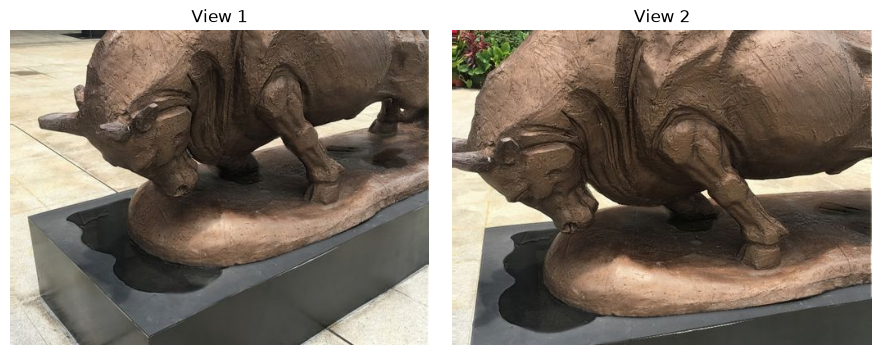
\includegraphics[width=0.9\textwidth]{figures/lesson29_fig01.png}
\caption{The two input views. \attrib{Image source: \href{https://github.com/YoYo000/BlendedMVS}{BlendedMVS} (CC BY 4.0).}}
\label{fig:l29-1}
\end{figure}

\section{An example}

\subsection*{Step 1: feature matching}

SIFT finds $504$ keypoints in view 1 and $654$ in view 2; Lowe's ratio test keeps $64$ good matches, shown in Figure~\ref{fig:l29-2}.

\begin{figure}[h]
\centering
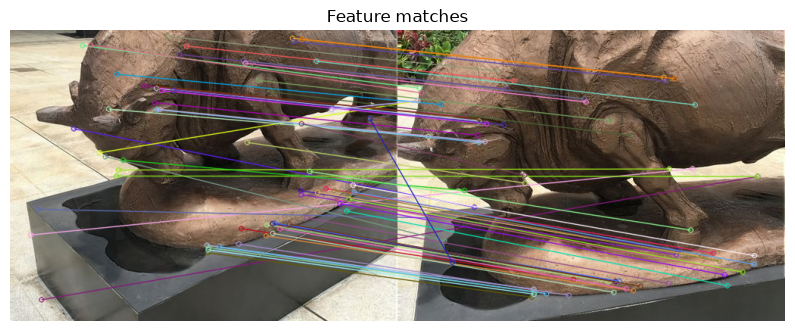
\includegraphics[width=0.9\textwidth]{figures/lesson29_fig02.png}
\caption{Feature matches between the two views.}
\label{fig:l29-2}
\end{figure}

\subsection*{Step 2: robust essential matrix and pose recovery}

Feed the matched points through the same robust pipeline built in Chapters~\ref{ch:lesson23} and \ref{ch:lesson27} to recover the essential matrix and the cameras' relative pose: $48$ of $64$ matches pass as RANSAC inliers. The recovered rotation matches the true rotation closely (e.g.\ $0.9245$ vs.\ true $0.9208$ for the leading diagonal entry), and the recovered translation direction ($-0.9967, 0.0791, 0.0174$) is close to the true direction ($-0.999, 0.0125, 0.0427$). As before, \code{recoverPose} returns only a \textbf{unit-length} translation direction --- the baseline distance is fundamentally unrecoverable from image correspondences alone.

\subsection*{Step 3: triangulation}

Given two camera projection matrices $P_1,P_2$ (each $3\times4$) and a matched pixel pair $(x_1,x_2)$, find the 3D point $X$ satisfying both $x_1\propto P_1X$ and $x_2\propto P_2X$. Each view contributes 2 independent linear equations in $X$'s 4 homogeneous unknowns, by the same DLT/SVD recipe used for homographies (Chapter~\ref{ch:lesson24}) and the fundamental matrix (Chapter~\ref{ch:lesson28}):
\begin{equation}
A = \begin{bmatrix} u_1 P_1^{(3)} - P_1^{(1)} \\ v_1 P_1^{(3)} - P_1^{(2)} \\ u_2 P_2^{(3)} - P_2^{(1)} \\ v_2 P_2^{(3)} - P_2^{(2)} \end{bmatrix}, \qquad AX = 0,
\end{equation}
where $P^{(i)}$ denotes row $i$ of $P$; the null space of $A$ gives $X$. A from-scratch DLT triangulation matches \code{cv2.triangulatePoints} to $10^{-7}$.

\subsection*{Cheirality: a free sanity check}

Decomposing $E$ into $(R,t)$ actually yields four mathematically valid sign combinations; only one places the observed points in front of \emph{both} cameras, and \code{cv2.recoverPose} uses exactly this \textbf{cheirality constraint} to pick the right one internally. The epipolar constraint alone doesn't rule out a correspondence that triangulates \emph{behind} a camera, so a mismatched point can still pass RANSAC's inlier test; requiring positive depth in both views is a free extra filter --- it drops the reconstruction from $48$ to $47$ inliers here. Triangulating those 47 points with the \emph{true} camera poses gives a mean reprojection error of just $0.169$ px (max $1.680$ px).

\section{Putting it together: reconstruction using estimated pose}

The real test: triangulate using the camera matrix built from \code{recoverPose}'s \emph{estimated} $(R,t)$, not the dataset's true pose. Because $t$ was only recovered up to scale, so is the reconstruction --- every 3D point comes out a fixed factor smaller than reality. Multiplying by the true baseline length ($0.788$, a bit of cheating, just for evaluation) recovers the correct metric scene: mean 3D reconstruction error (vs.\ triangulation from the true poses) is just $0.058$, max $0.096$ --- a small fraction of the baseline.

With real (imperfect) correspondences, the entire pipeline --- essential matrix, pose, triangulation --- reconstructs the scene to within a small fraction of the camera baseline, using nothing but 2D pixel correspondences and known intrinsics, plus \emph{one} external number (the true baseline) to fix the scale ambiguity. In practice, that scale reference might come from a known object size in the scene, a second sensor (GPS, IMU, LiDAR), or a calibrated stereo rig (Chapter~\ref{ch:lesson22}) instead of two arbitrary independent cameras.

\subsection*{Visualizing the reconstruction}

Loosening the feature-matching thresholds pulls in more (slightly noisier) correspondences for a denser cloud: $112$ points, colored by their pixel color from view 1, shown in Figure~\ref{fig:l29-3}.

\begin{figure}[h]
\centering
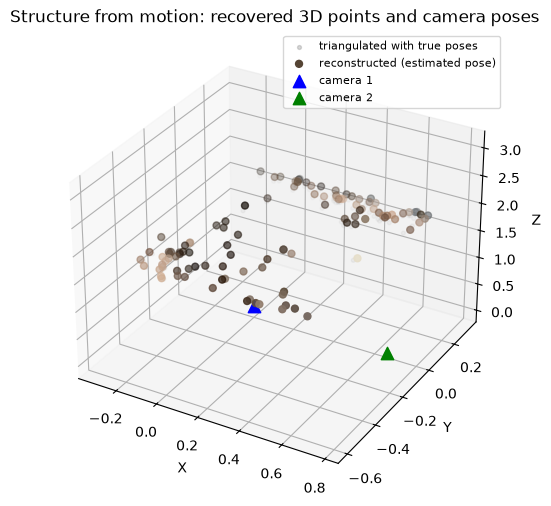
\includegraphics[width=0.6\textwidth]{figures/lesson29_fig03.png}
\caption{The recovered 3D points (colored, estimated pose) alongside points triangulated with the true poses (gray), plus both camera centers.}
\label{fig:l29-3}
\end{figure}

\subsection*{From sparse to dense, and from two views to many}

Even with loosened thresholds, feature matching only yields a \emph{sparse} cloud --- one 3D point per distinctive keypoint. With camera poses known, \textbf{multi-view stereo (MVS)} estimates a depth for \emph{every} pixel in \emph{every} view (a generalization of Chapter~\ref{ch:lesson22}'s stereo matching to arbitrarily-posed calibrated cameras), and those per-view depth maps are fused into the dense colored point cloud or mesh that toolkits like COLMAP (\citelink{schonberger2016colmap}{Sch\"onberger \& Frahm, 2016}) produce.

Real reconstructions rarely stop at two views. The standard recipe sequentially incorporates new images: match features against existing images, compute the new camera's pose relative to the existing 3D point cloud (Perspective-n-Point, \code{cv2.solvePnP}), then update the cloud by triangulation. As views accumulate, errors compound --- pose corrupts triangulated points, which corrupt the next recovered pose, and so on. \textbf{Bundle adjustment} fixes this by refining all camera poses and 3D points \emph{together} in one large nonlinear least-squares optimization that minimizes total reprojection error across every point in every view at once --- arguably the single most important step separating a simple two-view pipeline like this chapter's from a real SfM system.

\subsection*{Exercises}
\begin{enumerate}
  \item Add extra synthetic pixel noise on top of the already-real detections before triangulating. How much does the reconstruction error grow, and does it grow uniformly, or worse for points farther from the cameras (Chapter~\ref{ch:lesson22}'s disparity-depth relationship: distant points produce smaller, noisier parallax)?
  \item Sketch, in words, how you'd extend this notebook to a third view using \code{cv2.solvePnP}: which 3D points from the two-view reconstruction would you match into the new image, and how would \code{solvePnP}'s inputs and outputs map onto the pieces already in hand ($K$, matched 2D points, the existing 3D point cloud)?
  \item This pair has a deliberately generous baseline for reliable matching. How would you expect a much shorter baseline to affect the number of RANSAC inliers, and the accuracy of the recovered pose and reconstruction, compared to the wide-baseline pair used above?
\end{enumerate}

\vfill
\fullcode{lesson29}{lesson29_structure_from_motion}
